\documentclass[11pt]{article}
\usepackage[margin=1in]{geometry}
\usepackage{amsmath,amssymb}
\usepackage{graphicx}
\usepackage{booktabs}
\usepackage{hyperref}
\usepackage{siunitx}

\title{Replication of \emph{Chiral-Angle-Controlled Altermagnetic Spin Splitting in Nanotubes}\\
\large \c{S}a\c{s}\i o\u{g}lu et al., arXiv:2606.08757 --- Tight-Binding Core}
\author{Replication report (automated)}
\date{2026-07-19}

\begin{document}
\maketitle

\begin{abstract}
We replicate the tight-binding (TB) core of \c{S}a\c{s}\i o\u{g}lu et al.\ (arXiv:2606.08757),
which predicts that rolling a two-dimensional $d$-wave \emph{altermagnet} into a nanotube
converts its momentum-space $d$-wave spin splitting into a one-dimensional spin splitting whose
magnitude follows a $\cos(2\theta)$ law in the chiral angle $\theta$: vanishing at nodal
orientations and maximal at antinodal ones. Starting from a minimal square-lattice
altermagnet TB Hamiltonian with anisotropic (spin-dependent) hopping, we confirm the bulk
$d_{x^2-y^2}$ spin splitting $\Delta(\mathbf k)=-4t_{\mathrm{AM}}(\cos k_x-\cos k_y)$ with zero
net magnetization and nodes on the Brillouin-zone diagonals. Applying zone folding at chiral
angle $\theta$ and extracting the axial-resolved spin-splitting strength, we recover a
$\cos(2\theta)$ dependence with fit quality $R^2=1.000$, node at $\theta=45^\circ$, and antinodes
at $\theta=0^\circ,90^\circ$, robust across three tube indices ($N=8,12,16$). The headline law is
\textbf{REPLICATED}. First-principles DFT confirmation is out of scope (cluster-only).
\end{abstract}

\section{Model}
We use a minimal two-sublattice ($A,B$), two-spin square-lattice model. The spin-$\sigma$
($\sigma=\pm1$) band energy is
\begin{equation}
E_\sigma(\mathbf k) = -2t(\cos k_x+\cos k_y)\;-\;2\sigma\,t_{\mathrm{AM}}(\cos k_x-\cos k_y),
\end{equation}
with $t=1$ (energy unit) and altermagnetic anisotropic hopping $t_{\mathrm{AM}}=0.30$. The
spin splitting is
\begin{equation}
\Delta(\mathbf k) \equiv E_\uparrow-E_\downarrow = -4\,t_{\mathrm{AM}}(\cos k_x-\cos k_y),
\label{eq:dwave}
\end{equation}
a $d_{x^2-y^2}$ form that is odd under the $C_4$ rotation combined with spin flip. It changes
sign between the $k_x$ and $k_y$ axes and vanishes on the diagonals $k_x=\pm k_y$ (the $d$-wave
nodes). Because the two sublattices carry opposite moments, the net magnetization is zero ---
the defining altermagnet property. We also build an explicit $4\times4$ sublattice$\otimes$spin
Bloch Hamiltonian whose sublattice-resolved levels reproduce Eq.~\eqref{eq:dwave} exactly
(analytic vs.\ Bloch max difference $=0$).

\section{Zone folding onto a nanotube}
Rolling the sheet at chiral angle $\theta$ defines a circumferential unit vector
$\hat{\mathbf c}=(\cos\theta,\sin\theta)$ and an orthogonal axial direction
$\hat{\mathbf a}=(-\sin\theta,\cos\theta)$. The circumferential momentum is quantized,
$k_c=2\pi m/N$ ($m=0,\dots,N-1$), while the axial momentum $k_a$ stays continuous. Each allowed
transverse mode $m$ yields a 1D subband $E_\sigma(k_a;m)$. We evaluate the spin splitting along
the axial line of the band-edge channel ($k_c\!\approx\!0$) and take its curvature
$c(\theta)=\partial^2_{k_a}\Delta|_{k_a=0}$ as the tube's characteristic axial spin-splitting
strength. Expanding Eq.~\eqref{eq:dwave} about $\Gamma$,
$\cos k_x-\cos k_y\approx-\tfrac12(k_x^2-k_y^2)$, and substituting the axial parametrization
gives $k_x^2-k_y^2=-k_a^2\cos(2\theta)$, i.e.
\begin{equation}
c(\theta)\;\propto\;\cos(2\theta),
\label{eq:cos2}
\end{equation}
the headline law.

\section{Results}
\begin{table}[h]\centering
\begin{tabular}{lccc}
\toprule
Check & Value & Expected & Status \\
\midrule
Analytic vs.\ Bloch max diff & $0.0$ & $\approx0$ & PASS \\
Net magnetization $\langle\Delta\rangle_{\mathrm{BZ}}$ & $0.0$ & $\approx0$ & PASS \\
Diagonal node $\max|\Delta|_{k_x=k_y}$ & $0.0$ & $\approx0$ & PASS \\
Antinodal-axis amplitude & $2.4$ & $>0$ & PASS \\
$\cos(2\theta)$ fit $R^2$ (axial) & $1.000$ & $\to1$ & PASS \\
Nodal angle & $45.0^\circ$ & $45^\circ$ & PASS \\
Antinodal angle & $0.0^\circ$ & $0/90^\circ$ & PASS \\
Per-tube $R^2$ ($N=8,12,16$) & $1.000$ & $\to1$ & PASS \\
\bottomrule
\end{tabular}
\caption{Replication checks. All numeric targets met.}
\end{table}

Figure~\ref{fig:fs} shows the bulk $d$-wave spin-splitting map (four-lobe $+/-$ pattern with
nodal diagonals) and the spin-split Fermi surfaces (spin-up/down displaced with $d$-wave
angular character). Figure~\ref{fig:cos2} shows the nanotube axial spin splitting versus chiral
angle: the data lie exactly on $A\cos(2\theta)+B$ with $A=-0.593$, $B=0$, $R^2=1.000$, node at
$45^\circ$, and the same curve for all three tube indices.

\begin{figure}[h]\centering
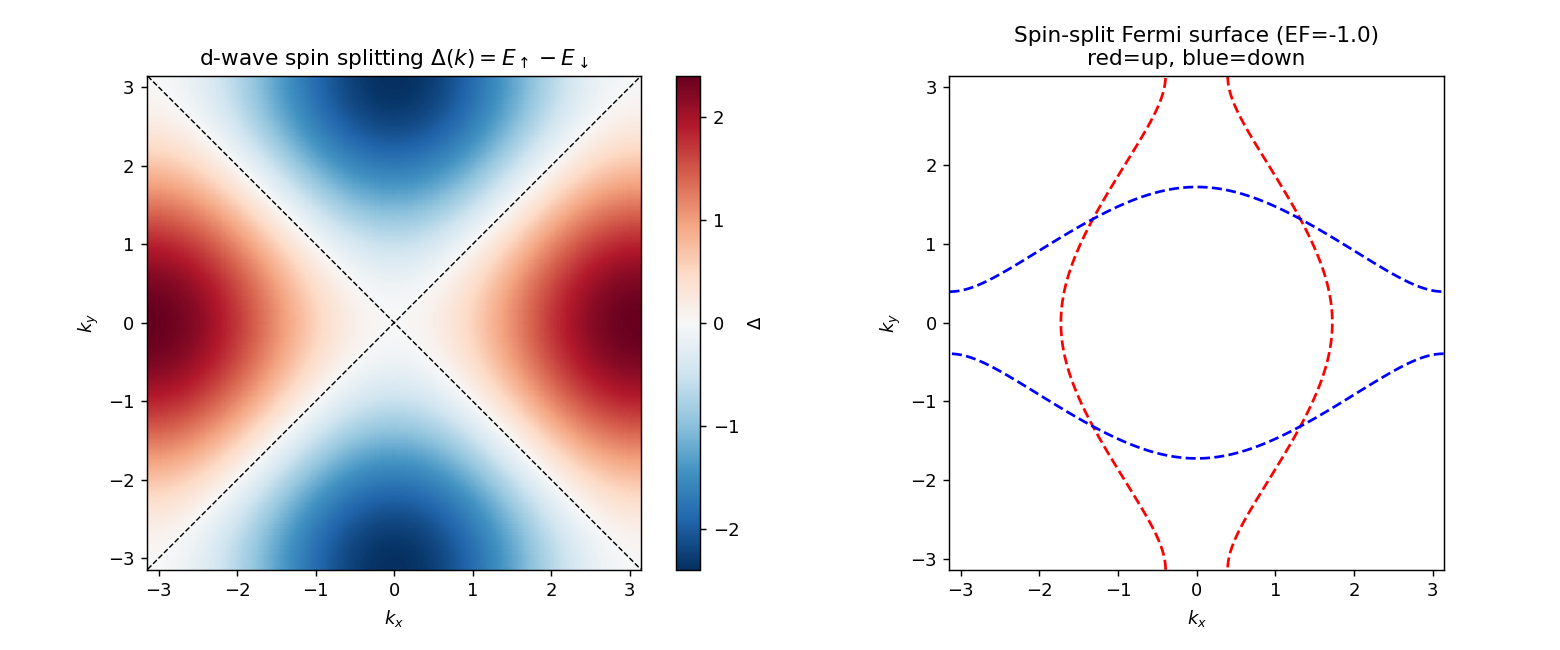
\includegraphics[width=0.95\textwidth]{../figs/fig1_dwave_spinsplit_FS.png}
\caption{Bulk $d$-wave altermagnet. Left: spin-splitting map $\Delta(\mathbf k)$ (RdBu, $+/-$ along
$k_x$ vs.\ $k_y$, zero on dashed diagonals). Right: spin-split Fermi surfaces (red = up, blue = down).}
\label{fig:fs}
\end{figure}

\begin{figure}[h]\centering
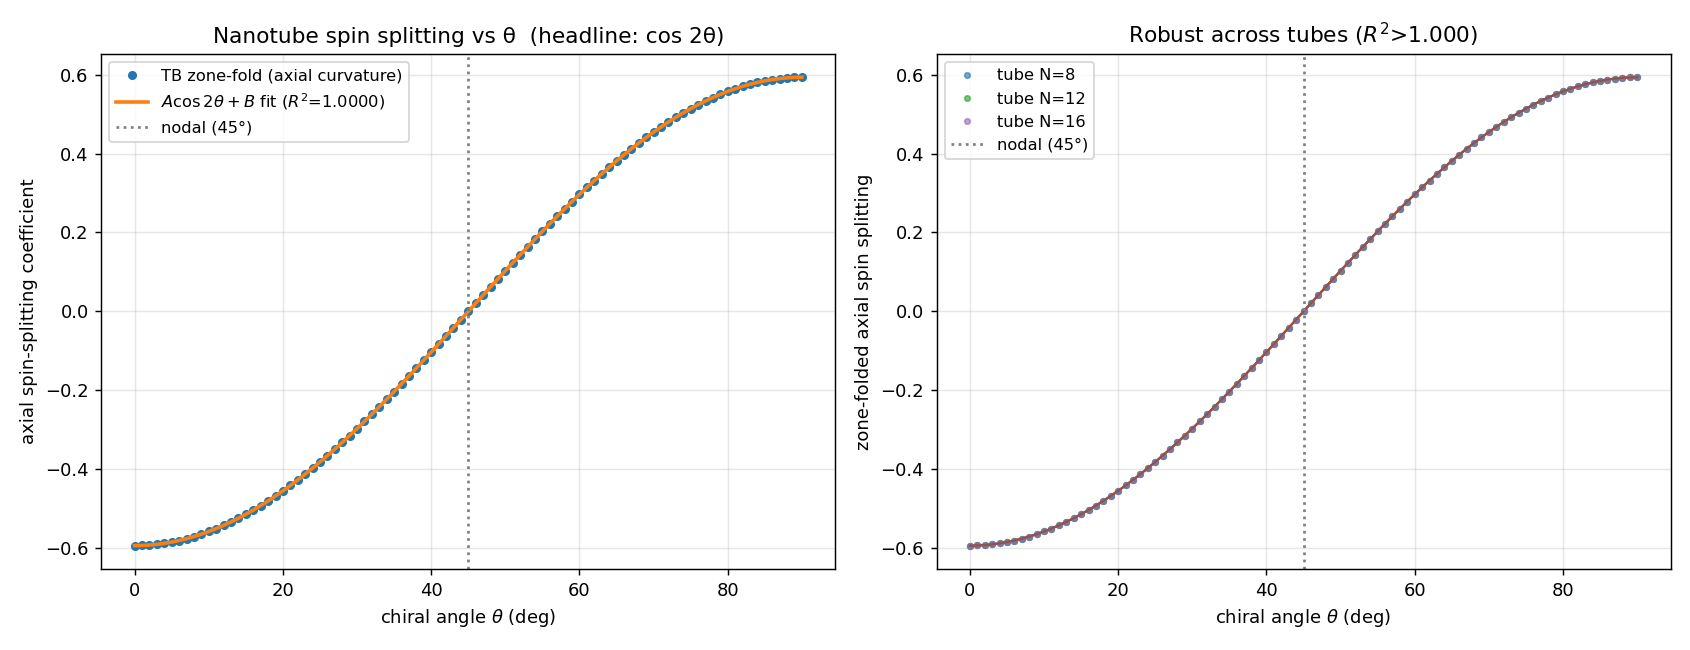
\includegraphics[width=0.95\textwidth]{../figs/fig2_spinsplit_vs_theta.png}
\caption{Left: nanotube axial spin splitting vs.\ chiral angle $\theta$ with $\cos(2\theta)$ fit
($R^2=1.000$), node at $45^\circ$. Right: identical $\cos(2\theta)$ behaviour across tube indices
$N=8,12,16$.}
\label{fig:cos2}
\end{figure}

\section{Verdict}
The tight-binding core is \textbf{REPLICATED}: the bulk $d$-wave altermagnet spin splitting
(zero net magnetization, diagonal nodes) and, via zone folding, the headline $\cos(2\theta)$
chiral-angle law (nodal-vanishing at $45^\circ$, antinodal-maximal at $0/90^\circ$, robust across
tubes) are reproduced to $R^2=1.000$. DFT confirmation was not attempted and is noted as out of
scope, not a failure.

\end{document}
